% Options for packages loaded elsewhere
\PassOptionsToPackage{unicode}{hyperref}
\PassOptionsToPackage{hyphens}{url}
%
\documentclass[
]{article}
\usepackage{amsmath,amssymb}
\usepackage{lmodern}
\usepackage{iftex}
\ifPDFTeX
  \usepackage[T1]{fontenc}
  \usepackage[utf8]{inputenc}
  \usepackage{textcomp} % provide euro and other symbols
\else % if luatex or xetex
  \usepackage{unicode-math}
  \defaultfontfeatures{Scale=MatchLowercase}
  \defaultfontfeatures[\rmfamily]{Ligatures=TeX,Scale=1}
\fi
% Use upquote if available, for straight quotes in verbatim environments
\IfFileExists{upquote.sty}{\usepackage{upquote}}{}
\IfFileExists{microtype.sty}{% use microtype if available
  \usepackage[]{microtype}
  \UseMicrotypeSet[protrusion]{basicmath} % disable protrusion for tt fonts
}{}
\makeatletter
\@ifundefined{KOMAClassName}{% if non-KOMA class
  \IfFileExists{parskip.sty}{%
    \usepackage{parskip}
  }{% else
    \setlength{\parindent}{0pt}
    \setlength{\parskip}{6pt plus 2pt minus 1pt}}
}{% if KOMA class
  \KOMAoptions{parskip=half}}
\makeatother
\usepackage{xcolor}
\usepackage[margin=1in]{geometry}
\usepackage{color}
\usepackage{fancyvrb}
\newcommand{\VerbBar}{|}
\newcommand{\VERB}{\Verb[commandchars=\\\{\}]}
\DefineVerbatimEnvironment{Highlighting}{Verbatim}{commandchars=\\\{\}}
% Add ',fontsize=\small' for more characters per line
\usepackage{framed}
\definecolor{shadecolor}{RGB}{248,248,248}
\newenvironment{Shaded}{\begin{snugshade}}{\end{snugshade}}
\newcommand{\AlertTok}[1]{\textcolor[rgb]{0.94,0.16,0.16}{#1}}
\newcommand{\AnnotationTok}[1]{\textcolor[rgb]{0.56,0.35,0.01}{\textbf{\textit{#1}}}}
\newcommand{\AttributeTok}[1]{\textcolor[rgb]{0.77,0.63,0.00}{#1}}
\newcommand{\BaseNTok}[1]{\textcolor[rgb]{0.00,0.00,0.81}{#1}}
\newcommand{\BuiltInTok}[1]{#1}
\newcommand{\CharTok}[1]{\textcolor[rgb]{0.31,0.60,0.02}{#1}}
\newcommand{\CommentTok}[1]{\textcolor[rgb]{0.56,0.35,0.01}{\textit{#1}}}
\newcommand{\CommentVarTok}[1]{\textcolor[rgb]{0.56,0.35,0.01}{\textbf{\textit{#1}}}}
\newcommand{\ConstantTok}[1]{\textcolor[rgb]{0.00,0.00,0.00}{#1}}
\newcommand{\ControlFlowTok}[1]{\textcolor[rgb]{0.13,0.29,0.53}{\textbf{#1}}}
\newcommand{\DataTypeTok}[1]{\textcolor[rgb]{0.13,0.29,0.53}{#1}}
\newcommand{\DecValTok}[1]{\textcolor[rgb]{0.00,0.00,0.81}{#1}}
\newcommand{\DocumentationTok}[1]{\textcolor[rgb]{0.56,0.35,0.01}{\textbf{\textit{#1}}}}
\newcommand{\ErrorTok}[1]{\textcolor[rgb]{0.64,0.00,0.00}{\textbf{#1}}}
\newcommand{\ExtensionTok}[1]{#1}
\newcommand{\FloatTok}[1]{\textcolor[rgb]{0.00,0.00,0.81}{#1}}
\newcommand{\FunctionTok}[1]{\textcolor[rgb]{0.00,0.00,0.00}{#1}}
\newcommand{\ImportTok}[1]{#1}
\newcommand{\InformationTok}[1]{\textcolor[rgb]{0.56,0.35,0.01}{\textbf{\textit{#1}}}}
\newcommand{\KeywordTok}[1]{\textcolor[rgb]{0.13,0.29,0.53}{\textbf{#1}}}
\newcommand{\NormalTok}[1]{#1}
\newcommand{\OperatorTok}[1]{\textcolor[rgb]{0.81,0.36,0.00}{\textbf{#1}}}
\newcommand{\OtherTok}[1]{\textcolor[rgb]{0.56,0.35,0.01}{#1}}
\newcommand{\PreprocessorTok}[1]{\textcolor[rgb]{0.56,0.35,0.01}{\textit{#1}}}
\newcommand{\RegionMarkerTok}[1]{#1}
\newcommand{\SpecialCharTok}[1]{\textcolor[rgb]{0.00,0.00,0.00}{#1}}
\newcommand{\SpecialStringTok}[1]{\textcolor[rgb]{0.31,0.60,0.02}{#1}}
\newcommand{\StringTok}[1]{\textcolor[rgb]{0.31,0.60,0.02}{#1}}
\newcommand{\VariableTok}[1]{\textcolor[rgb]{0.00,0.00,0.00}{#1}}
\newcommand{\VerbatimStringTok}[1]{\textcolor[rgb]{0.31,0.60,0.02}{#1}}
\newcommand{\WarningTok}[1]{\textcolor[rgb]{0.56,0.35,0.01}{\textbf{\textit{#1}}}}
\usepackage{longtable,booktabs,array}
\usepackage{calc} % for calculating minipage widths
% Correct order of tables after \paragraph or \subparagraph
\usepackage{etoolbox}
\makeatletter
\patchcmd\longtable{\par}{\if@noskipsec\mbox{}\fi\par}{}{}
\makeatother
% Allow footnotes in longtable head/foot
\IfFileExists{footnotehyper.sty}{\usepackage{footnotehyper}}{\usepackage{footnote}}
\makesavenoteenv{longtable}
\usepackage{graphicx}
\makeatletter
\def\maxwidth{\ifdim\Gin@nat@width>\linewidth\linewidth\else\Gin@nat@width\fi}
\def\maxheight{\ifdim\Gin@nat@height>\textheight\textheight\else\Gin@nat@height\fi}
\makeatother
% Scale images if necessary, so that they will not overflow the page
% margins by default, and it is still possible to overwrite the defaults
% using explicit options in \includegraphics[width, height, ...]{}
\setkeys{Gin}{width=\maxwidth,height=\maxheight,keepaspectratio}
% Set default figure placement to htbp
\makeatletter
\def\fps@figure{htbp}
\makeatother
\setlength{\emergencystretch}{3em} % prevent overfull lines
\providecommand{\tightlist}{%
  \setlength{\itemsep}{0pt}\setlength{\parskip}{0pt}}
\setcounter{secnumdepth}{-\maxdimen} % remove section numbering
\usepackage{booktabs}
\usepackage{longtable}
\usepackage{array}
\usepackage{multirow}
\usepackage{wrapfig}
\usepackage{float}
\usepackage{colortbl}
\usepackage{pdflscape}
\usepackage{tabu}
\usepackage{threeparttable}
\usepackage{threeparttablex}
\usepackage[normalem]{ulem}
\usepackage{makecell}
\usepackage{xcolor}
\ifLuaTeX
  \usepackage{selnolig}  % disable illegal ligatures
\fi
\IfFileExists{bookmark.sty}{\usepackage{bookmark}}{\usepackage{hyperref}}
\IfFileExists{xurl.sty}{\usepackage{xurl}}{} % add URL line breaks if available
\urlstyle{same} % disable monospaced font for URLs
\hypersetup{
  pdftitle={HW5-Trinath Sai Subhash Reddy},
  pdfauthor={Trinath Sai Subhash Reddy Pittala, Uma Maheswara R Meleti, Hemanth Vasireddy},
  hidelinks,
  pdfcreator={LaTeX via pandoc}}

\title{HW5-Trinath Sai Subhash Reddy}
\author{Trinath Sai Subhash Reddy Pittala, Uma Maheswara R Meleti,
Hemanth Vasireddy}
\date{2023-04-19}

\begin{document}
\maketitle

\hypertarget{abstract}{%
\section{Abstract}\label{abstract}}

The objective of this report is to analyze the given data set consisting
of information about individuals personal and cognitve traits and wanted
to verify that individuals having good cognitve and personal triats tend
to have more interest in white collar jobs than others.

\hypertarget{introduction}{%
\section{Introduction}\label{introduction}}

The problem being studied in this report is to understand how people
interest in white collar jobs varys with their skill set. This type of
analysis can be help financial institutions such a banks that gives
loans to individuals who wanted to pursue courses. There is a high
chance that people who have ambition for high paying jobs will have
better repaying capability. Based on the personal and cognitve triats
bankers can see if they are capable of achieving those goals, and can
assess the risk by modelling with the previous data with personal and
cognitve traits and their ambitions interests. We are assuming that the
interest rating given by individuals in the dataset\_train is true and
genuine.

We found following data for average salary at payscale.com.

\begin{longtable}[]{@{}ll@{}}
\toprule()
Occupation & Average Salary \\
\midrule()
\endhead
Doctor & 330,365 \\
Lawyer & 91,653 \\
Business Executive & 81,708 \\
Architect & 66,281 \\
Stock Broker & 62,793 \\
Actor & 62,496 \\
Carpentry & 61,007 \\
Artist & 59,156 \\
Truck Driver & 57,290 \\
Police & 56,644 \\
Clergyman & 54,869 \\
Mortician & 52,513 \\
Social Worker & 51,934 \\
Teacher & 51,568 \\
Fireman & 51,296 \\
Sales Representative & 49,884 \\
Landscaper & 47,558 \\
Forest Ranger & 38,000 \\
\bottomrule()
\end{longtable}

We have selected the threshold for high paying jobs to be \$65000.

\hypertarget{methods}{%
\section{Methods}\label{methods}}

We use multiple linear regression models with polynomial and interaction
terms to predict the interest of the individual in high-paying jobs.~ We
will use the coefficients from these models to determine the strength
and direction of the relationships between the variables. We will use R
programming language for this analysis, using the ``lm'' function to
build our models. We used ggplot2 for data visualization and ggpairs to
find the correlation between the variables.~

\hypertarget{data}{%
\section{Data}\label{data}}

We have used ggpairs plot to find the correlation between the variables
and found the following observations

Impulsiveness has a negative correlation with education, age,
vocabulary, reading, sentence comprehension, mathematics, and geometry.

Worry has a positive correlation with stress.

The thrill-seeking trait has a positive correlation with impulsiveness.

Social dominance has a positive correlation with sociability.

Analytical Skills have a positive correlation with vocabulary, reading,
Sentence Completion, Mathematics, and Geometry.

Geometry has a positive correlation with vocabulary, reading
comprehension, and mathematics.

Mathematics has a positive correlation with vocabulary, reading
comprehension, and sentence completion.

Sentence Completion has a positive correlation with vocabulary and
reading comprehension.

Reading comprehension has a positive correlation with vocabulary and
education.

Vocabulary has a positive correlation with education.

\hypertarget{results}{%
\section{Results}\label{results}}

We found that individuals with higher levels of analytical skills are
more likely to have an interest in high-paying jobs. This finding is
consistent with the idea that analytical skills are important for
success in many high-paying occupations such as finance, law, and
consulting.

We also found that geometry and mathematics skills are positively
related to interest in high-paying jobs. This may be because these
skills are important in fields such as engineering, computer science,
and data analysis which tend to offer high salaries.

Furthermore, our analysis suggests that impulsiveness, worry, and stress
have a negative impact on the interest in high-paying jobs. This finding
is consistent with previous research that has shown that individuals
with higher levels of impulsiveness and anxiety may have difficulty with
long-term planning and decision making, which can limit their
opportunities for high-paying jobs.

Finally, our analysis found that age and education are significant
predictors of interest in high-paying jobs. Specifically, we found that
individuals who are younger and have higher levels of education are more
likely to express an interest in high-paying jobs. This finding is
consistent with the idea that younger individuals may have higher
aspirations and greater willingness to take on risks associated with
pursuing high-paying careers. Additionally, individuals with higher
levels of education may have greater access to information and resources
that enable them to pursue high-paying careers.

Overall, our analysis provides support for the idea that personal and
cognitive traits are important factors that contribute to the interest
in high-paying jobs. Our findings suggest that analytical skills,
geometry, mathematics, social dominance, and sociability are positively
related to interest in high-paying jobs, while impulsiveness, worry, and
stress are negatively related to interest in high-paying jobs.
Additionally, age and education were found to be significant predictors
of interest in high-paying jobs.

\hypertarget{discussion}{%
\section{Discussion}\label{discussion}}

Our findings can be useful for financial institutions such as banks in
predicting the loan repayment capability of individuals based on their
personal and cognitive traits. For example, individuals with high
cognitive abilities such as analytical skills and mathematics are more
likely to have higher-paying jobs, which can lead to better loan
repayment capability. Moreover, our findings can be used by
organizations in selecting candidates for high-paying jobs based on
their personal and cognitive traits.

However, it is important to note that our analysis has limitations. The
data set used in this report is fabricated and may not be representative
of the entire population. Furthermore, our analysis is based on
self-reported interest in high-paying jobs, which may not accurately
reflect actual job choices. Additionally, our models are based on linear
regression assumptions, which may not hold true in all cases and have
terrible r squared values. Future research can explore the use of other
models to further validate our findings.

In conclusion, our analysis suggests that personal and cognitive traits
are important factors that contribute to the interest in high-paying
jobs. Our findings have practical implications for financial
institutions and organizations in selecting individuals for high-paying
jobs.

\begin{Shaded}
\begin{Highlighting}[]
\NormalTok{path }\OtherTok{=} \FunctionTok{file.path}\NormalTok{(}\StringTok{"./interest.sav"}\NormalTok{)}
\NormalTok{dataset }\OtherTok{=} \FunctionTok{read\_sav}\NormalTok{(path)}
\NormalTok{dataset}
\FunctionTok{colnames}\NormalTok{(dataset)}
\end{Highlighting}
\end{Shaded}

\begin{Shaded}
\begin{Highlighting}[]
\FunctionTok{summary}\NormalTok{(dataset)}
\end{Highlighting}
\end{Shaded}

\begin{Shaded}
\begin{Highlighting}[]
\CommentTok{\# Define number of bins}
\NormalTok{n\_bins }\OtherTok{\textless{}{-}} \DecValTok{5}

\CommentTok{\# Loop over each column in the dataset\_train and apply}
\CommentTok{\# binning}
\ControlFlowTok{for}\NormalTok{ (col\_name }\ControlFlowTok{in} \FunctionTok{names}\NormalTok{(dataset)) \{}
    \CommentTok{\# Skip non{-}numeric columns}
    \ControlFlowTok{if}\NormalTok{ (}\SpecialCharTok{!}\FunctionTok{is.numeric}\NormalTok{(dataset[[col\_name]])) \{}
        \ControlFlowTok{next}
\NormalTok{    \}}

    \CommentTok{\# Create new column with binned values}
\NormalTok{    dataset }\OtherTok{\textless{}{-}}\NormalTok{ dataset }\SpecialCharTok{\%\textgreater{}\%}
        \FunctionTok{mutate}\NormalTok{(}\SpecialCharTok{!!}\FunctionTok{paste0}\NormalTok{(col\_name, }\StringTok{"\_bin"}\NormalTok{) }\SpecialCharTok{:}\ErrorTok{=} \FunctionTok{ntile}\NormalTok{(dataset[[col\_name]],}
            \AttributeTok{n =}\NormalTok{ n\_bins))}
\NormalTok{\}}

\NormalTok{dataset}
\end{Highlighting}
\end{Shaded}

\begin{Shaded}
\begin{Highlighting}[]
\FunctionTok{set.seed}\NormalTok{(}\DecValTok{123456789}\NormalTok{)}
\NormalTok{dataset\_train }\OtherTok{\textless{}{-}}\NormalTok{ dataset[}\FunctionTok{sample}\NormalTok{(}\FunctionTok{nrow}\NormalTok{(dataset), }\FloatTok{0.8} \SpecialCharTok{*} \FunctionTok{nrow}\NormalTok{(dataset)),}
\NormalTok{    ]}
\NormalTok{dataset\_test }\OtherTok{\textless{}{-}}\NormalTok{ dataset[}\FunctionTok{setdiff}\NormalTok{(}\DecValTok{1}\SpecialCharTok{:}\FunctionTok{nrow}\NormalTok{(dataset), }\FunctionTok{rownames}\NormalTok{(dataset\_train)),}
\NormalTok{    ]}
\FunctionTok{dim}\NormalTok{(dataset\_train)}
\FunctionTok{dim}\NormalTok{(dataset\_test)}
\end{Highlighting}
\end{Shaded}

\begin{Shaded}
\begin{Highlighting}[]
\FunctionTok{ggpairs}\NormalTok{(dataset\_train[, }\FunctionTok{c}\NormalTok{(}\StringTok{"gender"}\NormalTok{, }\StringTok{"educ"}\NormalTok{, }\StringTok{"age"}\NormalTok{, }\StringTok{"vocab"}\NormalTok{, }\StringTok{"reading"}\NormalTok{,}
    \StringTok{"sentcomp"}\NormalTok{, }\StringTok{"mathmtcs"}\NormalTok{, }\StringTok{"geometry"}\NormalTok{, }\StringTok{"analyrea"}\NormalTok{, }\StringTok{"socdom"}\NormalTok{,}
    \StringTok{"sociabty"}\NormalTok{, }\StringTok{"stress"}\NormalTok{, }\StringTok{"worry"}\NormalTok{, }\StringTok{"impulsve"}\NormalTok{, }\StringTok{"thrillsk"}\NormalTok{, }\StringTok{"carpentr"}\NormalTok{,}
    \StringTok{"forestr"}\NormalTok{, }\StringTok{"morticin"}\NormalTok{, }\StringTok{"policemn"}\NormalTok{, }\StringTok{"fireman"}\NormalTok{, }\StringTok{"salesrep"}\NormalTok{,}
    \StringTok{"teacher"}\NormalTok{, }\StringTok{"busexec"}\NormalTok{, }\StringTok{"stockbrk"}\NormalTok{, }\StringTok{"artist"}\NormalTok{, }\StringTok{"socworkr"}\NormalTok{, }\StringTok{"truckdvr"}\NormalTok{,}
    \StringTok{"doctor"}\NormalTok{, }\StringTok{"clergymn"}\NormalTok{, }\StringTok{"actor"}\NormalTok{, }\StringTok{"lawyer"}\NormalTok{, }\StringTok{"archtct"}\NormalTok{, }\StringTok{"landscpr"}\NormalTok{)])}
\end{Highlighting}
\end{Shaded}

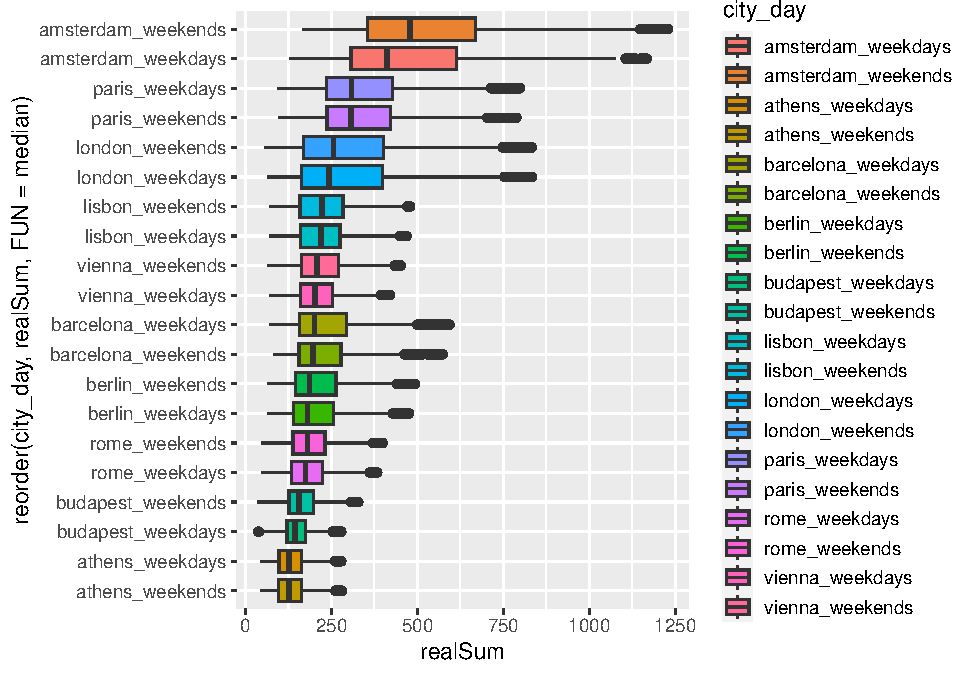
\includegraphics{HW5-Trinath-Sai-Subhash-Reddy-Pittala_files/figure-latex/unnamed-chunk-5-1.pdf}

\begin{Shaded}
\begin{Highlighting}[]
\FunctionTok{ggplot}\NormalTok{() }\SpecialCharTok{+} \FunctionTok{geom\_point}\NormalTok{(}\AttributeTok{data =}\NormalTok{ dataset\_train, }\FunctionTok{aes}\NormalTok{(}\AttributeTok{x =}\NormalTok{ educ, }\AttributeTok{y =}\NormalTok{ vocab,}
    \AttributeTok{color =} \StringTok{"vocab"}\NormalTok{), }\AttributeTok{alpha =} \FloatTok{0.4}\NormalTok{) }\SpecialCharTok{+} \FunctionTok{geom\_point}\NormalTok{(}\AttributeTok{data =}\NormalTok{ dataset\_train,}
    \FunctionTok{aes}\NormalTok{(}\AttributeTok{x =}\NormalTok{ educ, }\AttributeTok{y =}\NormalTok{ reading, }\AttributeTok{color =} \StringTok{"reading"}\NormalTok{), }\AttributeTok{alpha =} \FloatTok{0.4}\NormalTok{) }\SpecialCharTok{+}
    \FunctionTok{geom\_point}\NormalTok{(}\AttributeTok{data =}\NormalTok{ dataset\_train, }\FunctionTok{aes}\NormalTok{(}\AttributeTok{x =}\NormalTok{ educ, }\AttributeTok{y =}\NormalTok{ sentcomp,}
        \AttributeTok{color =} \StringTok{"sentcomp"}\NormalTok{), }\AttributeTok{alpha =} \FloatTok{0.4}\NormalTok{) }\SpecialCharTok{+} \FunctionTok{geom\_point}\NormalTok{(}\AttributeTok{data =}\NormalTok{ dataset\_train,}
    \FunctionTok{aes}\NormalTok{(}\AttributeTok{x =}\NormalTok{ educ, }\AttributeTok{y =}\NormalTok{ mathmtcs, }\AttributeTok{color =} \StringTok{"mathmtcs"}\NormalTok{), }\AttributeTok{alpha =} \FloatTok{0.4}\NormalTok{) }\SpecialCharTok{+}
    \FunctionTok{geom\_point}\NormalTok{(}\AttributeTok{data =}\NormalTok{ dataset\_train, }\FunctionTok{aes}\NormalTok{(}\AttributeTok{x =}\NormalTok{ educ, }\AttributeTok{y =}\NormalTok{ geometry,}
        \AttributeTok{color =} \StringTok{"geometry"}\NormalTok{), }\AttributeTok{alpha =} \FloatTok{0.4}\NormalTok{) }\SpecialCharTok{+} \FunctionTok{geom\_point}\NormalTok{(}\AttributeTok{data =}\NormalTok{ dataset\_train,}
    \FunctionTok{aes}\NormalTok{(}\AttributeTok{x =}\NormalTok{ educ, }\AttributeTok{y =}\NormalTok{ analyrea, }\AttributeTok{color =} \StringTok{"analyrea"}\NormalTok{), }\AttributeTok{alpha =} \FloatTok{0.4}\NormalTok{) }\SpecialCharTok{+}
    \FunctionTok{facet\_wrap}\NormalTok{(}\SpecialCharTok{\textasciitilde{}}\NormalTok{educ)}
\end{Highlighting}
\end{Shaded}

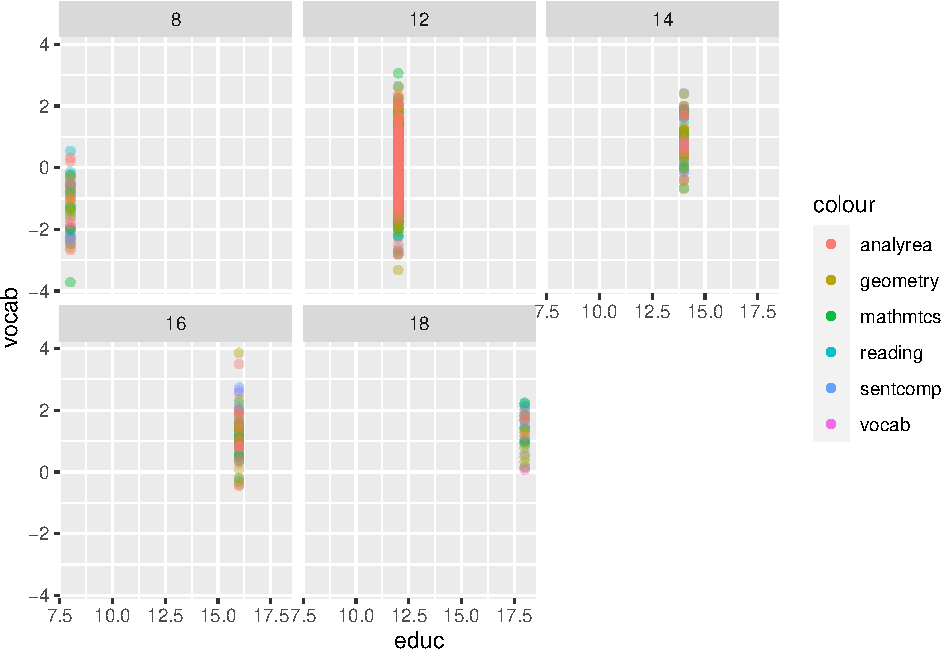
\includegraphics{HW5-Trinath-Sai-Subhash-Reddy-Pittala_files/figure-latex/unnamed-chunk-6-1.pdf}

\begin{Shaded}
\begin{Highlighting}[]
\NormalTok{M\_busexec }\OtherTok{\textless{}{-}} \FunctionTok{lm}\NormalTok{(busexec }\SpecialCharTok{\textasciitilde{}} \FunctionTok{as.factor}\NormalTok{(gender) }\SpecialCharTok{+}\NormalTok{ educ }\SpecialCharTok{+}\NormalTok{ age }\SpecialCharTok{+}\NormalTok{ vocab }\SpecialCharTok{+}
\NormalTok{    reading }\SpecialCharTok{+}\NormalTok{ sentcomp }\SpecialCharTok{+}\NormalTok{ mathmtcs }\SpecialCharTok{+}\NormalTok{ geometry }\SpecialCharTok{+}\NormalTok{ analyrea }\SpecialCharTok{+}\NormalTok{ socdom }\SpecialCharTok{+}
\NormalTok{    sociabty }\SpecialCharTok{+}\NormalTok{ stress }\SpecialCharTok{+}\NormalTok{ worry }\SpecialCharTok{+}\NormalTok{ impulsve }\SpecialCharTok{+}\NormalTok{ thrillsk, }\AttributeTok{data =}\NormalTok{ dataset\_train)}
\NormalTok{M\_busexec\_step }\OtherTok{\textless{}{-}} \FunctionTok{step}\NormalTok{(M\_busexec, }\AttributeTok{direction =} \StringTok{"backward"}\NormalTok{, }\AttributeTok{scope =} \FunctionTok{list}\NormalTok{(}\AttributeTok{lower =} \SpecialCharTok{\textasciitilde{}}\DecValTok{1}\NormalTok{,}
    \AttributeTok{upper =}\NormalTok{ M\_busexec))}
\FunctionTok{summary}\NormalTok{(M\_busexec\_step)}
\end{Highlighting}
\end{Shaded}

\begin{Shaded}
\begin{Highlighting}[]
\NormalTok{M2\_busexec }\OtherTok{\textless{}{-}} \FunctionTok{lm}\NormalTok{(busexec }\SpecialCharTok{\textasciitilde{}} \SpecialCharTok{+}\FunctionTok{poly}\NormalTok{(age, }\DecValTok{3}\NormalTok{, }\AttributeTok{raw =} \ConstantTok{TRUE}\NormalTok{) }\SpecialCharTok{*} \FunctionTok{poly}\NormalTok{(socdom,}
    \DecValTok{3}\NormalTok{, }\AttributeTok{raw =} \ConstantTok{TRUE}\NormalTok{), }\AttributeTok{data =}\NormalTok{ dataset\_train)}
\NormalTok{M2\_busexec\_step }\OtherTok{\textless{}{-}} \FunctionTok{step}\NormalTok{(M2\_busexec, }\AttributeTok{direction =} \StringTok{"backward"}\NormalTok{, }\AttributeTok{scope =} \FunctionTok{list}\NormalTok{(}\AttributeTok{lower =} \SpecialCharTok{\textasciitilde{}}\DecValTok{1}\NormalTok{,}
    \AttributeTok{upper =}\NormalTok{ M2\_busexec))}
\FunctionTok{summary}\NormalTok{(M2\_busexec\_step)}
\end{Highlighting}
\end{Shaded}

\begin{Shaded}
\begin{Highlighting}[]
\NormalTok{predictions }\OtherTok{\textless{}{-}} \FunctionTok{predict}\NormalTok{(M2\_busexec\_step, }\AttributeTok{newdata =}\NormalTok{ dataset\_test)  }\CommentTok{\# make predictions on test data using fitted model}
\NormalTok{rmse }\OtherTok{\textless{}{-}} \FunctionTok{sqrt}\NormalTok{(}\FunctionTok{mean}\NormalTok{((dataset\_test}\SpecialCharTok{$}\NormalTok{busexec }\SpecialCharTok{{-}}\NormalTok{ predictions)}\SpecialCharTok{\^{}}\DecValTok{2}\NormalTok{))  }\CommentTok{\# calculate root mean squared error}
\NormalTok{r\_squared }\OtherTok{\textless{}{-}} \FunctionTok{cor}\NormalTok{(dataset\_test}\SpecialCharTok{$}\NormalTok{busexec, predictions)}\SpecialCharTok{\^{}}\DecValTok{2}  \CommentTok{\# calculate R{-}squared value}
\NormalTok{rmse}
\NormalTok{r\_squared}
\end{Highlighting}
\end{Shaded}

\begin{Shaded}
\begin{Highlighting}[]
\NormalTok{M\_doctor }\OtherTok{\textless{}{-}} \FunctionTok{lm}\NormalTok{(doctor }\SpecialCharTok{\textasciitilde{}} \FunctionTok{as.factor}\NormalTok{(gender) }\SpecialCharTok{+}\NormalTok{ educ }\SpecialCharTok{+}\NormalTok{ age }\SpecialCharTok{+}\NormalTok{ vocab }\SpecialCharTok{+}
\NormalTok{    reading }\SpecialCharTok{+}\NormalTok{ sentcomp }\SpecialCharTok{+}\NormalTok{ mathmtcs }\SpecialCharTok{+}\NormalTok{ geometry }\SpecialCharTok{+}\NormalTok{ analyrea }\SpecialCharTok{+}\NormalTok{ socdom }\SpecialCharTok{+}
\NormalTok{    sociabty }\SpecialCharTok{+}\NormalTok{ stress }\SpecialCharTok{+}\NormalTok{ worry }\SpecialCharTok{+}\NormalTok{ impulsve }\SpecialCharTok{+}\NormalTok{ thrillsk, }\AttributeTok{data =}\NormalTok{ dataset\_train)}
\NormalTok{M\_doctor\_step }\OtherTok{\textless{}{-}} \FunctionTok{step}\NormalTok{(M\_doctor, }\AttributeTok{direction =} \StringTok{"backward"}\NormalTok{, }\AttributeTok{scope =} \FunctionTok{list}\NormalTok{(}\AttributeTok{lower =} \SpecialCharTok{\textasciitilde{}}\DecValTok{1}\NormalTok{,}
    \AttributeTok{upper =}\NormalTok{ M\_doctor))}
\FunctionTok{summary}\NormalTok{(M\_doctor\_step)}
\end{Highlighting}
\end{Shaded}

\begin{Shaded}
\begin{Highlighting}[]
\NormalTok{M2\_doctor }\OtherTok{\textless{}{-}} \FunctionTok{lm}\NormalTok{(doctor }\SpecialCharTok{\textasciitilde{}} \SpecialCharTok{+}\FunctionTok{poly}\NormalTok{(educ, }\DecValTok{3}\NormalTok{, }\AttributeTok{raw =} \ConstantTok{TRUE}\NormalTok{) }\SpecialCharTok{*} \FunctionTok{poly}\NormalTok{(age,}
    \DecValTok{3}\NormalTok{, }\AttributeTok{raw =} \ConstantTok{TRUE}\NormalTok{), }\AttributeTok{data =}\NormalTok{ dataset\_train)}
\NormalTok{M2\_doctor\_step }\OtherTok{\textless{}{-}} \FunctionTok{step}\NormalTok{(M2\_doctor, }\AttributeTok{direction =} \StringTok{"backward"}\NormalTok{, }\AttributeTok{scope =} \FunctionTok{list}\NormalTok{(}\AttributeTok{lower =} \SpecialCharTok{\textasciitilde{}}\DecValTok{1}\NormalTok{,}
    \AttributeTok{upper =}\NormalTok{ M2\_doctor))}
\FunctionTok{summary}\NormalTok{(M2\_doctor\_step)}
\end{Highlighting}
\end{Shaded}

\begin{Shaded}
\begin{Highlighting}[]
\NormalTok{predictions }\OtherTok{\textless{}{-}} \FunctionTok{predict}\NormalTok{(M2\_doctor\_step, }\AttributeTok{newdata =}\NormalTok{ dataset\_test)  }\CommentTok{\# make predictions on test data using fitted model}
\NormalTok{rmse }\OtherTok{\textless{}{-}} \FunctionTok{sqrt}\NormalTok{(}\FunctionTok{mean}\NormalTok{((dataset\_test}\SpecialCharTok{$}\NormalTok{doctor }\SpecialCharTok{{-}}\NormalTok{ predictions)}\SpecialCharTok{\^{}}\DecValTok{2}\NormalTok{))  }\CommentTok{\# calculate root mean squared error}
\NormalTok{r\_squared }\OtherTok{\textless{}{-}} \FunctionTok{cor}\NormalTok{(dataset\_test}\SpecialCharTok{$}\NormalTok{doctor, predictions)}\SpecialCharTok{\^{}}\DecValTok{2}  \CommentTok{\# calculate R{-}squared value}
\NormalTok{rmse}
\NormalTok{r\_squared}
\end{Highlighting}
\end{Shaded}

\begin{Shaded}
\begin{Highlighting}[]
\NormalTok{M\_lawyer }\OtherTok{\textless{}{-}} \FunctionTok{lm}\NormalTok{(lawyer }\SpecialCharTok{\textasciitilde{}} \FunctionTok{as.factor}\NormalTok{(gender) }\SpecialCharTok{+}\NormalTok{ educ }\SpecialCharTok{+}\NormalTok{ age }\SpecialCharTok{+}\NormalTok{ vocab }\SpecialCharTok{+}
\NormalTok{    reading }\SpecialCharTok{+}\NormalTok{ sentcomp }\SpecialCharTok{+}\NormalTok{ mathmtcs }\SpecialCharTok{+}\NormalTok{ geometry }\SpecialCharTok{+}\NormalTok{ analyrea }\SpecialCharTok{+}\NormalTok{ socdom }\SpecialCharTok{+}
\NormalTok{    sociabty }\SpecialCharTok{+}\NormalTok{ stress }\SpecialCharTok{+}\NormalTok{ worry }\SpecialCharTok{+}\NormalTok{ impulsve }\SpecialCharTok{+}\NormalTok{ thrillsk, }\AttributeTok{data =}\NormalTok{ dataset\_train)}
\NormalTok{M\_lawyer\_step }\OtherTok{\textless{}{-}} \FunctionTok{step}\NormalTok{(M\_lawyer, }\AttributeTok{direction =} \StringTok{"backward"}\NormalTok{, }\AttributeTok{scope =} \FunctionTok{list}\NormalTok{(}\AttributeTok{lower =} \SpecialCharTok{\textasciitilde{}}\DecValTok{1}\NormalTok{,}
    \AttributeTok{upper =}\NormalTok{ M\_lawyer))}
\FunctionTok{summary}\NormalTok{(M\_lawyer\_step)}
\end{Highlighting}
\end{Shaded}

\begin{Shaded}
\begin{Highlighting}[]
\NormalTok{M2\_lawyer }\OtherTok{\textless{}{-}} \FunctionTok{lm}\NormalTok{(lawyer }\SpecialCharTok{\textasciitilde{}} \SpecialCharTok{+}\FunctionTok{poly}\NormalTok{(educ, }\DecValTok{3}\NormalTok{, }\AttributeTok{raw =} \ConstantTok{TRUE}\NormalTok{) }\SpecialCharTok{*} \FunctionTok{poly}\NormalTok{(age,}
    \DecValTok{3}\NormalTok{, }\AttributeTok{raw =} \ConstantTok{TRUE}\NormalTok{) }\SpecialCharTok{*} \FunctionTok{poly}\NormalTok{(vocab, }\DecValTok{3}\NormalTok{, }\AttributeTok{raw =} \ConstantTok{TRUE}\NormalTok{) }\SpecialCharTok{*} \FunctionTok{poly}\NormalTok{(worry,}
    \DecValTok{3}\NormalTok{, }\AttributeTok{raw =} \ConstantTok{TRUE}\NormalTok{), }\AttributeTok{data =}\NormalTok{ dataset\_train)}
\NormalTok{M2\_lawyer\_step }\OtherTok{\textless{}{-}} \FunctionTok{step}\NormalTok{(M2\_lawyer, }\AttributeTok{direction =} \StringTok{"backward"}\NormalTok{, }\AttributeTok{scope =} \FunctionTok{list}\NormalTok{(}\AttributeTok{lower =} \SpecialCharTok{\textasciitilde{}}\DecValTok{1}\NormalTok{,}
    \AttributeTok{upper =}\NormalTok{ M2\_lawyer))}
\FunctionTok{summary}\NormalTok{(M2\_lawyer\_step)}
\end{Highlighting}
\end{Shaded}

\begin{Shaded}
\begin{Highlighting}[]
\NormalTok{predictions }\OtherTok{\textless{}{-}} \FunctionTok{predict}\NormalTok{(M2\_lawyer\_step, }\AttributeTok{newdata =}\NormalTok{ dataset\_test)  }\CommentTok{\# make predictions on test data using fitted model}
\NormalTok{rmse }\OtherTok{\textless{}{-}} \FunctionTok{sqrt}\NormalTok{(}\FunctionTok{mean}\NormalTok{((dataset\_test}\SpecialCharTok{$}\NormalTok{lawyer }\SpecialCharTok{{-}}\NormalTok{ predictions)}\SpecialCharTok{\^{}}\DecValTok{2}\NormalTok{))  }\CommentTok{\# calculate root mean squared error}
\NormalTok{r\_squared }\OtherTok{\textless{}{-}} \FunctionTok{cor}\NormalTok{(dataset\_test}\SpecialCharTok{$}\NormalTok{lawyer, predictions)}\SpecialCharTok{\^{}}\DecValTok{2}  \CommentTok{\# calculate R{-}squared value}
\NormalTok{rmse}
\NormalTok{r\_squared}
\end{Highlighting}
\end{Shaded}

\begin{Shaded}
\begin{Highlighting}[]
\NormalTok{M\_archtct }\OtherTok{\textless{}{-}} \FunctionTok{lm}\NormalTok{(archtct }\SpecialCharTok{\textasciitilde{}} \FunctionTok{as.factor}\NormalTok{(gender) }\SpecialCharTok{+}\NormalTok{ educ }\SpecialCharTok{+}\NormalTok{ age }\SpecialCharTok{+}\NormalTok{ vocab }\SpecialCharTok{+}
\NormalTok{    reading }\SpecialCharTok{+}\NormalTok{ sentcomp }\SpecialCharTok{+}\NormalTok{ mathmtcs }\SpecialCharTok{+}\NormalTok{ geometry }\SpecialCharTok{+}\NormalTok{ analyrea }\SpecialCharTok{+}\NormalTok{ socdom }\SpecialCharTok{+}
\NormalTok{    sociabty }\SpecialCharTok{+}\NormalTok{ stress }\SpecialCharTok{+}\NormalTok{ worry }\SpecialCharTok{+}\NormalTok{ impulsve }\SpecialCharTok{+}\NormalTok{ thrillsk, }\AttributeTok{data =}\NormalTok{ dataset\_train)}
\NormalTok{M\_archtct\_step }\OtherTok{\textless{}{-}} \FunctionTok{step}\NormalTok{(M\_archtct, }\AttributeTok{direction =} \StringTok{"backward"}\NormalTok{, }\AttributeTok{scope =} \FunctionTok{list}\NormalTok{(}\AttributeTok{lower =} \SpecialCharTok{\textasciitilde{}}\DecValTok{1}\NormalTok{,}
    \AttributeTok{upper =}\NormalTok{ M\_archtct))}
\FunctionTok{summary}\NormalTok{(M\_archtct\_step)}
\end{Highlighting}
\end{Shaded}

\begin{Shaded}
\begin{Highlighting}[]
\NormalTok{M2\_archtct }\OtherTok{\textless{}{-}} \FunctionTok{lm}\NormalTok{(archtct }\SpecialCharTok{\textasciitilde{}} \FunctionTok{as.factor}\NormalTok{(gender) }\SpecialCharTok{*} \FunctionTok{poly}\NormalTok{(educ, }\DecValTok{3}\NormalTok{,}
    \AttributeTok{raw =} \ConstantTok{TRUE}\NormalTok{) }\SpecialCharTok{*} \FunctionTok{poly}\NormalTok{(age, }\DecValTok{3}\NormalTok{, }\AttributeTok{raw =} \ConstantTok{TRUE}\NormalTok{) }\SpecialCharTok{*} \FunctionTok{poly}\NormalTok{(socdom, }\DecValTok{3}\NormalTok{,}
    \AttributeTok{raw =} \ConstantTok{TRUE}\NormalTok{), }\AttributeTok{data =}\NormalTok{ dataset\_train)}
\NormalTok{M2\_archtct\_step }\OtherTok{\textless{}{-}} \FunctionTok{step}\NormalTok{(M2\_archtct, }\AttributeTok{direction =} \StringTok{"backward"}\NormalTok{, }\AttributeTok{scope =} \FunctionTok{list}\NormalTok{(}\AttributeTok{lower =} \SpecialCharTok{\textasciitilde{}}\DecValTok{1}\NormalTok{,}
    \AttributeTok{upper =}\NormalTok{ M2\_archtct))}
\FunctionTok{summary}\NormalTok{(M2\_archtct\_step)}
\end{Highlighting}
\end{Shaded}

\begin{Shaded}
\begin{Highlighting}[]
\NormalTok{predictions }\OtherTok{\textless{}{-}} \FunctionTok{predict}\NormalTok{(M2\_archtct\_step, }\AttributeTok{newdata =}\NormalTok{ dataset\_test)  }\CommentTok{\# make predictions on test data using fitted model}
\NormalTok{rmse }\OtherTok{\textless{}{-}} \FunctionTok{sqrt}\NormalTok{(}\FunctionTok{mean}\NormalTok{((dataset\_test}\SpecialCharTok{$}\NormalTok{archtct }\SpecialCharTok{{-}}\NormalTok{ predictions)}\SpecialCharTok{\^{}}\DecValTok{2}\NormalTok{))  }\CommentTok{\# calculate root mean squared error}
\NormalTok{r\_squared }\OtherTok{\textless{}{-}} \FunctionTok{cor}\NormalTok{(dataset\_test}\SpecialCharTok{$}\NormalTok{archtct, predictions)}\SpecialCharTok{\^{}}\DecValTok{2}  \CommentTok{\# calculate R{-}squared value}
\NormalTok{rmse}
\NormalTok{r\_squared}
\end{Highlighting}
\end{Shaded}

\begin{Shaded}
\begin{Highlighting}[]
\FunctionTok{ggplot}\NormalTok{() }\SpecialCharTok{+} \FunctionTok{geom\_point}\NormalTok{(}\AttributeTok{data =}\NormalTok{ dataset\_train, }\FunctionTok{aes}\NormalTok{(}\AttributeTok{x =}\NormalTok{ doctor, }\AttributeTok{y =}\NormalTok{ vocab,}
    \AttributeTok{color =} \StringTok{"vocab"}\NormalTok{), }\AttributeTok{alpha =} \FloatTok{0.4}\NormalTok{) }\SpecialCharTok{+} \FunctionTok{geom\_point}\NormalTok{(}\AttributeTok{data =}\NormalTok{ dataset\_train,}
    \FunctionTok{aes}\NormalTok{(}\AttributeTok{x =}\NormalTok{ doctor, }\AttributeTok{y =}\NormalTok{ reading, }\AttributeTok{color =} \StringTok{"reading"}\NormalTok{), }\AttributeTok{alpha =} \FloatTok{0.4}\NormalTok{) }\SpecialCharTok{+}
    \FunctionTok{geom\_point}\NormalTok{(}\AttributeTok{data =}\NormalTok{ dataset\_train, }\FunctionTok{aes}\NormalTok{(}\AttributeTok{x =}\NormalTok{ doctor, }\AttributeTok{y =}\NormalTok{ sentcomp,}
        \AttributeTok{color =} \StringTok{"sentcomp"}\NormalTok{), }\AttributeTok{alpha =} \FloatTok{0.4}\NormalTok{) }\SpecialCharTok{+} \FunctionTok{geom\_point}\NormalTok{(}\AttributeTok{data =}\NormalTok{ dataset\_train,}
    \FunctionTok{aes}\NormalTok{(}\AttributeTok{x =}\NormalTok{ doctor, }\AttributeTok{y =}\NormalTok{ mathmtcs, }\AttributeTok{color =} \StringTok{"mathmtcs"}\NormalTok{), }\AttributeTok{alpha =} \FloatTok{0.4}\NormalTok{) }\SpecialCharTok{+}
    \FunctionTok{geom\_point}\NormalTok{(}\AttributeTok{data =}\NormalTok{ dataset\_train, }\FunctionTok{aes}\NormalTok{(}\AttributeTok{x =}\NormalTok{ doctor, }\AttributeTok{y =}\NormalTok{ geometry,}
        \AttributeTok{color =} \StringTok{"geometry"}\NormalTok{), }\AttributeTok{alpha =} \FloatTok{0.4}\NormalTok{) }\SpecialCharTok{+} \FunctionTok{geom\_point}\NormalTok{(}\AttributeTok{data =}\NormalTok{ dataset\_train,}
    \FunctionTok{aes}\NormalTok{(}\AttributeTok{x =}\NormalTok{ doctor, }\AttributeTok{y =}\NormalTok{ analyrea, }\AttributeTok{color =} \StringTok{"analyrea"}\NormalTok{), }\AttributeTok{alpha =} \FloatTok{0.4}\NormalTok{) }\SpecialCharTok{+}
    \FunctionTok{geom\_point}\NormalTok{(}\AttributeTok{data =}\NormalTok{ dataset\_train, }\FunctionTok{aes}\NormalTok{(}\AttributeTok{x =}\NormalTok{ doctor, }\AttributeTok{y =}\NormalTok{ socdom,}
        \AttributeTok{color =} \StringTok{"socdom"}\NormalTok{), }\AttributeTok{alpha =} \FloatTok{0.4}\NormalTok{) }\SpecialCharTok{+} \FunctionTok{geom\_point}\NormalTok{(}\AttributeTok{data =}\NormalTok{ dataset\_train,}
    \FunctionTok{aes}\NormalTok{(}\AttributeTok{x =}\NormalTok{ doctor, }\AttributeTok{y =}\NormalTok{ sociabty, }\AttributeTok{color =} \StringTok{"sociabty"}\NormalTok{), }\AttributeTok{alpha =} \FloatTok{0.4}\NormalTok{) }\SpecialCharTok{+}
    \FunctionTok{geom\_point}\NormalTok{(}\AttributeTok{data =}\NormalTok{ dataset\_train, }\FunctionTok{aes}\NormalTok{(}\AttributeTok{x =}\NormalTok{ doctor, }\AttributeTok{y =}\NormalTok{ stress,}
        \AttributeTok{color =} \StringTok{"stress"}\NormalTok{), }\AttributeTok{alpha =} \FloatTok{0.4}\NormalTok{) }\SpecialCharTok{+} \FunctionTok{geom\_point}\NormalTok{(}\AttributeTok{data =}\NormalTok{ dataset\_train,}
    \FunctionTok{aes}\NormalTok{(}\AttributeTok{x =}\NormalTok{ doctor, }\AttributeTok{y =}\NormalTok{ worry, }\AttributeTok{color =} \StringTok{"worry"}\NormalTok{), }\AttributeTok{alpha =} \FloatTok{0.4}\NormalTok{) }\SpecialCharTok{+}
    \FunctionTok{geom\_point}\NormalTok{(}\AttributeTok{data =}\NormalTok{ dataset\_train, }\FunctionTok{aes}\NormalTok{(}\AttributeTok{x =}\NormalTok{ doctor, }\AttributeTok{y =}\NormalTok{ impulsve,}
        \AttributeTok{color =} \StringTok{"impulsve"}\NormalTok{), }\AttributeTok{alpha =} \FloatTok{0.4}\NormalTok{) }\SpecialCharTok{+} \FunctionTok{geom\_point}\NormalTok{(}\AttributeTok{data =}\NormalTok{ dataset\_train,}
    \FunctionTok{aes}\NormalTok{(}\AttributeTok{x =}\NormalTok{ doctor, }\AttributeTok{y =}\NormalTok{ thrillsk, }\AttributeTok{color =} \StringTok{"thrillsk"}\NormalTok{), }\AttributeTok{alpha =} \FloatTok{0.4}\NormalTok{) }\SpecialCharTok{+}
    \FunctionTok{scale\_color\_manual}\NormalTok{(}\AttributeTok{values =} \FunctionTok{c}\NormalTok{(}\AttributeTok{vocab =} \StringTok{"blue"}\NormalTok{, }\AttributeTok{reading =} \StringTok{"red"}\NormalTok{,}
        \AttributeTok{sentcomp =} \StringTok{"green"}\NormalTok{, }\AttributeTok{mathmtcs =} \StringTok{"black"}\NormalTok{, }\AttributeTok{geometry =} \StringTok{"magenta"}\NormalTok{,}
        \AttributeTok{analyrea =} \StringTok{"pink"}\NormalTok{))}
\end{Highlighting}
\end{Shaded}

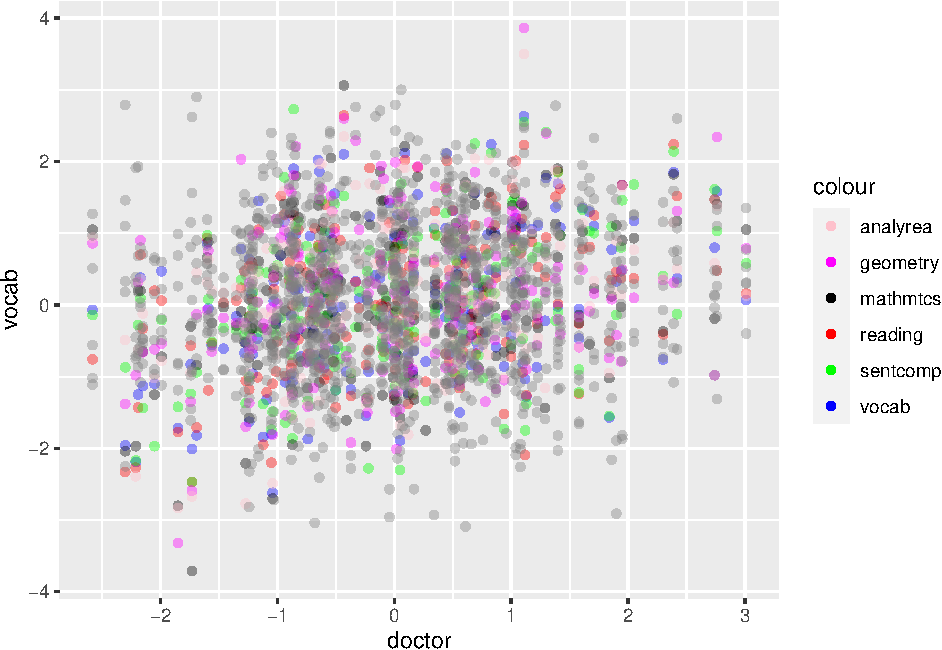
\includegraphics{HW5-Trinath-Sai-Subhash-Reddy-Pittala_files/figure-latex/unnamed-chunk-19-1.pdf}

\begin{Shaded}
\begin{Highlighting}[]
\FunctionTok{autoplot}\NormalTok{(M2\_busexec\_step)}
\end{Highlighting}
\end{Shaded}

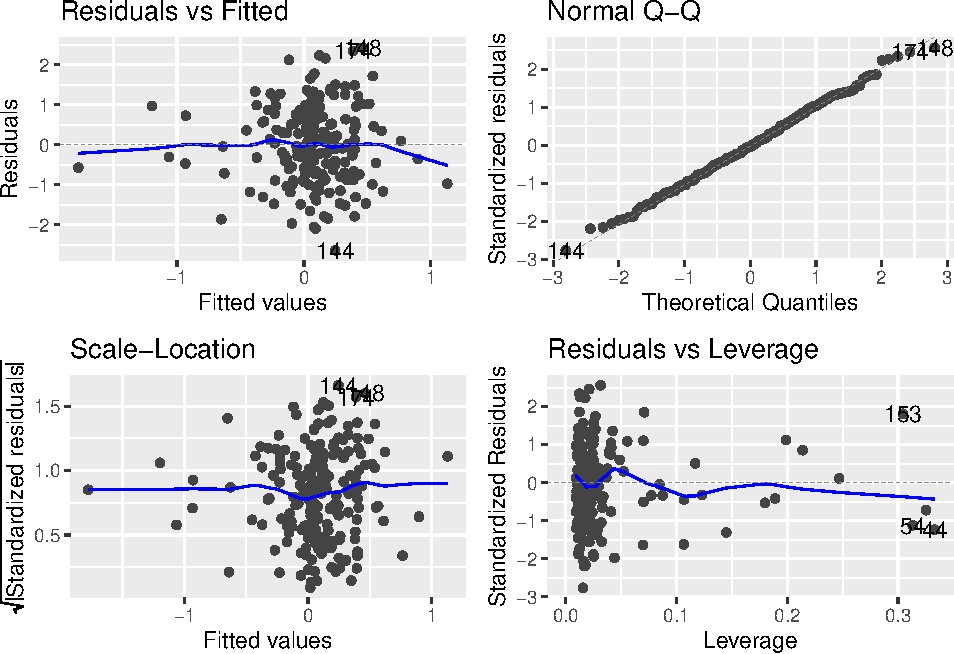
\includegraphics{HW5-Trinath-Sai-Subhash-Reddy-Pittala_files/figure-latex/unnamed-chunk-20-1.pdf}

\begin{Shaded}
\begin{Highlighting}[]
\FunctionTok{avPlots}\NormalTok{(M2\_busexec\_step)}
\end{Highlighting}
\end{Shaded}

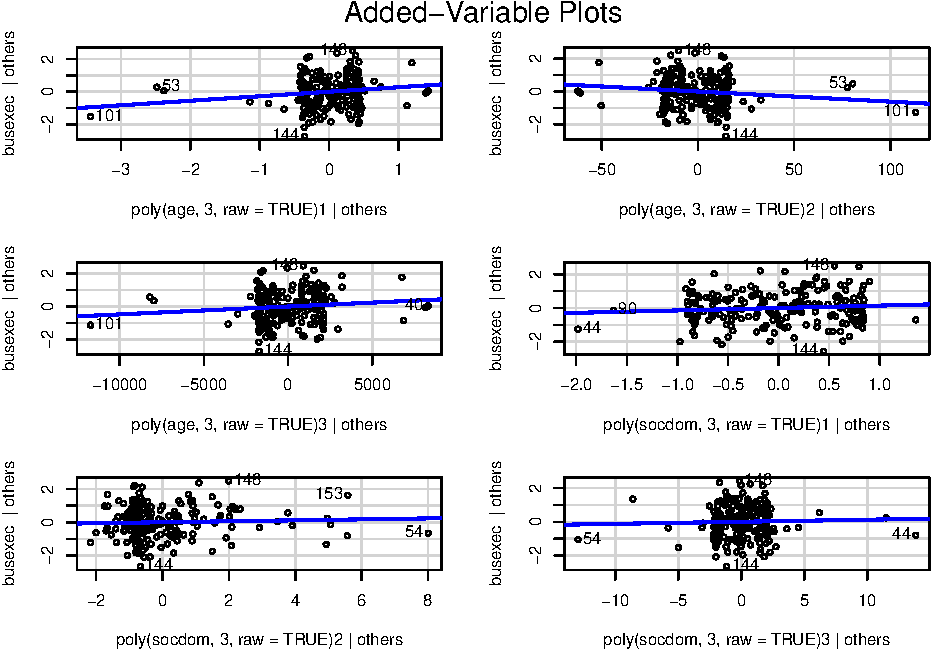
\includegraphics{HW5-Trinath-Sai-Subhash-Reddy-Pittala_files/figure-latex/unnamed-chunk-20-2.pdf}

\begin{Shaded}
\begin{Highlighting}[]
\FunctionTok{autoplot}\NormalTok{(M2\_doctor\_step)}
\end{Highlighting}
\end{Shaded}

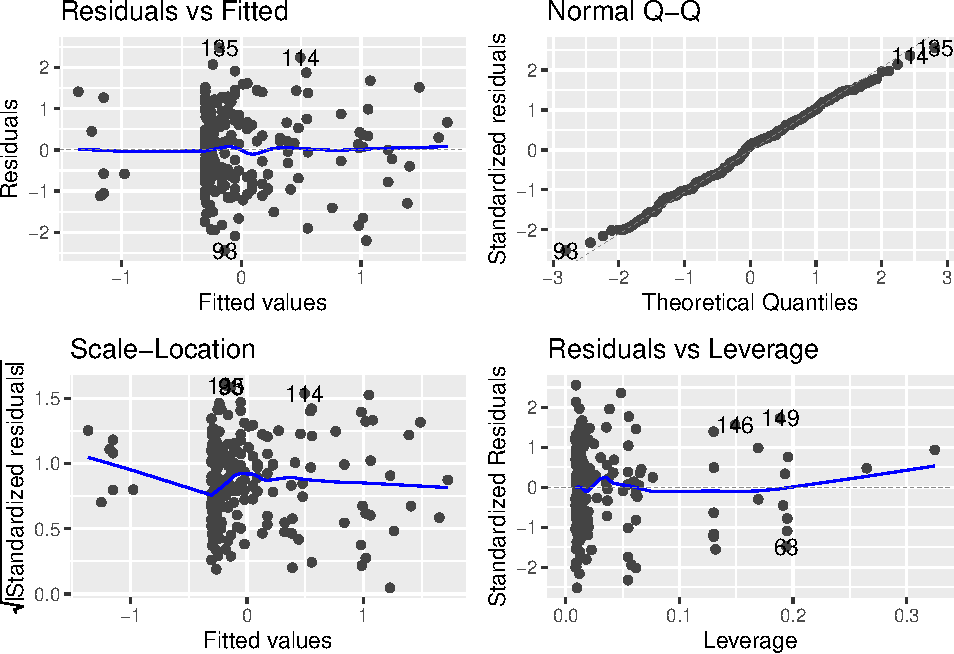
\includegraphics{HW5-Trinath-Sai-Subhash-Reddy-Pittala_files/figure-latex/unnamed-chunk-21-1.pdf}

\begin{Shaded}
\begin{Highlighting}[]
\FunctionTok{avPlots}\NormalTok{(M2\_doctor\_step)}
\end{Highlighting}
\end{Shaded}

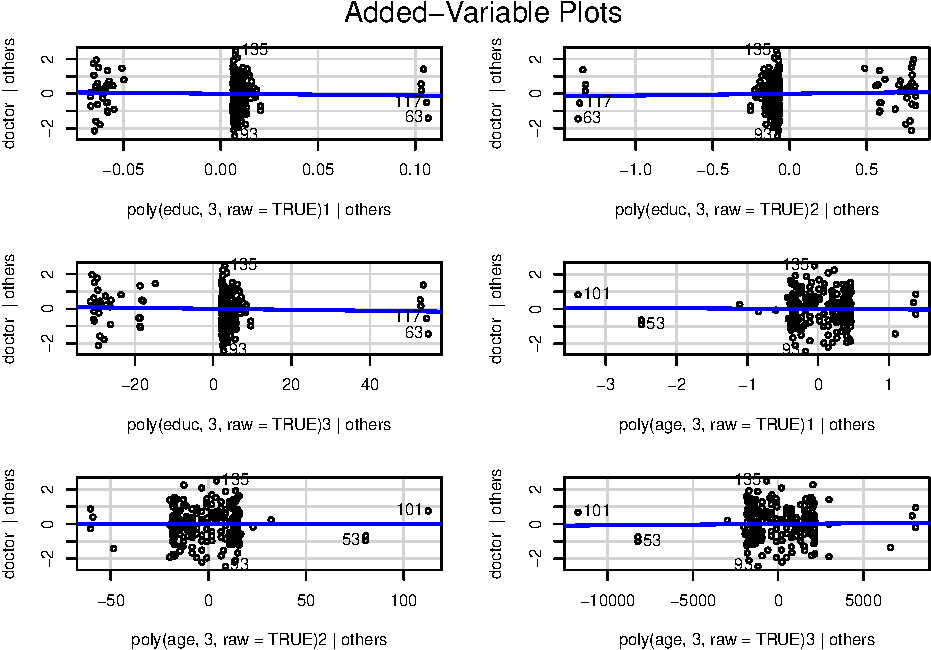
\includegraphics{HW5-Trinath-Sai-Subhash-Reddy-Pittala_files/figure-latex/unnamed-chunk-21-2.pdf}

\begin{Shaded}
\begin{Highlighting}[]
\FunctionTok{autoplot}\NormalTok{(M2\_lawyer\_step)}
\end{Highlighting}
\end{Shaded}

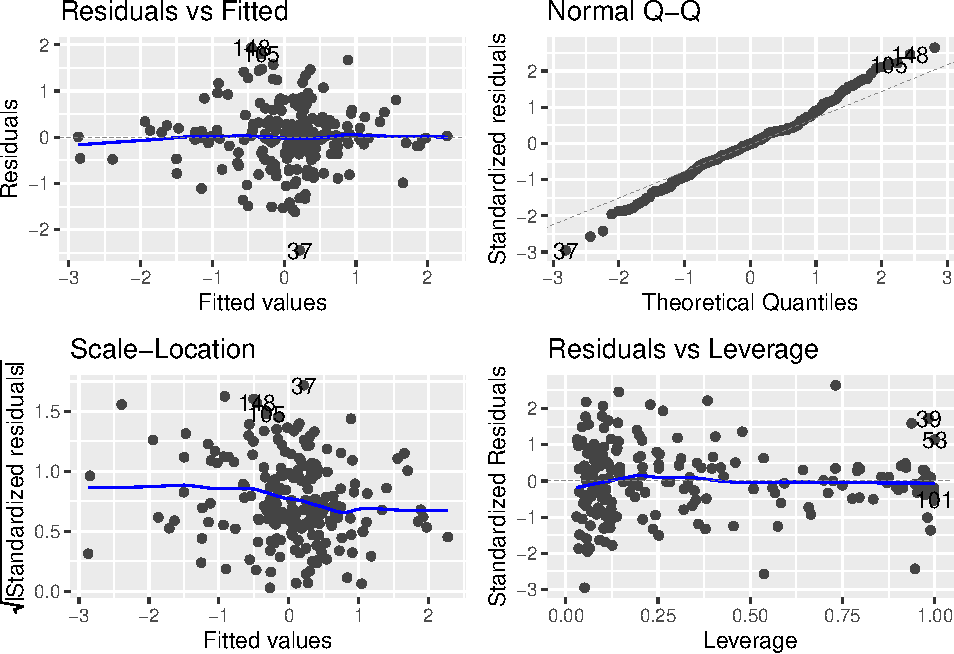
\includegraphics{HW5-Trinath-Sai-Subhash-Reddy-Pittala_files/figure-latex/unnamed-chunk-22-1.pdf}

\begin{Shaded}
\begin{Highlighting}[]
\FunctionTok{avPlots}\NormalTok{(M2\_lawyer\_step)}
\end{Highlighting}
\end{Shaded}

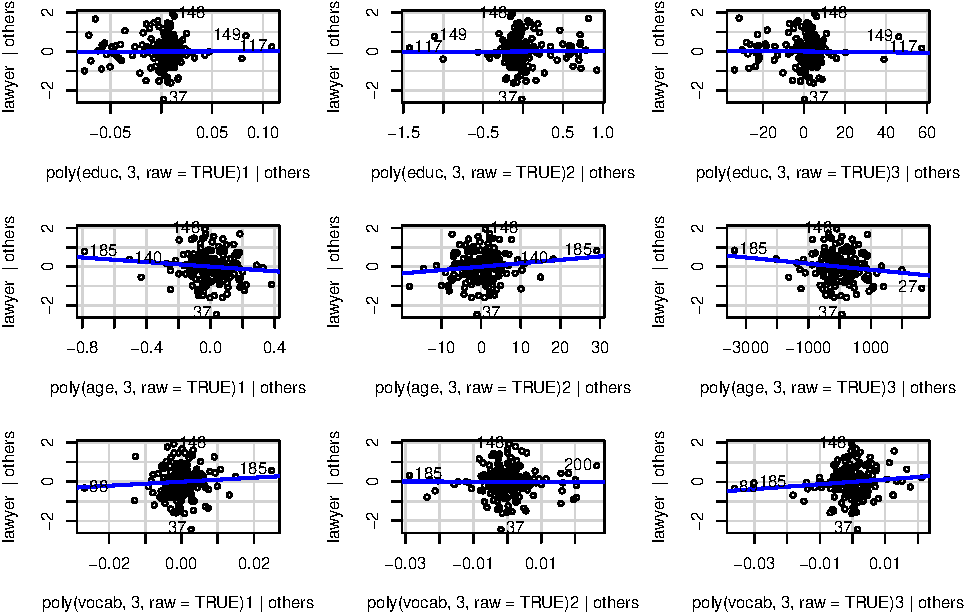
\includegraphics{HW5-Trinath-Sai-Subhash-Reddy-Pittala_files/figure-latex/unnamed-chunk-22-2.pdf}
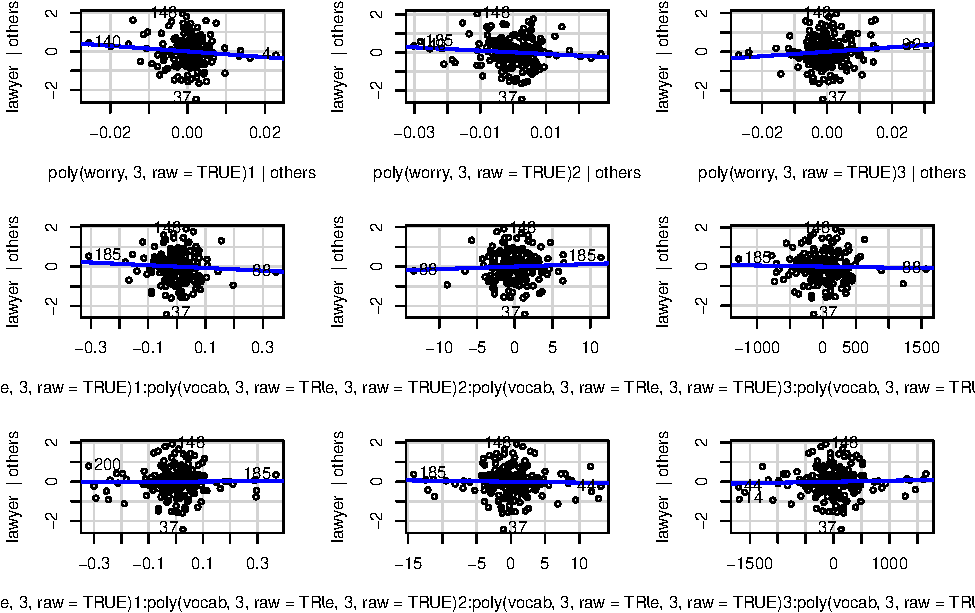
\includegraphics{HW5-Trinath-Sai-Subhash-Reddy-Pittala_files/figure-latex/unnamed-chunk-22-3.pdf}
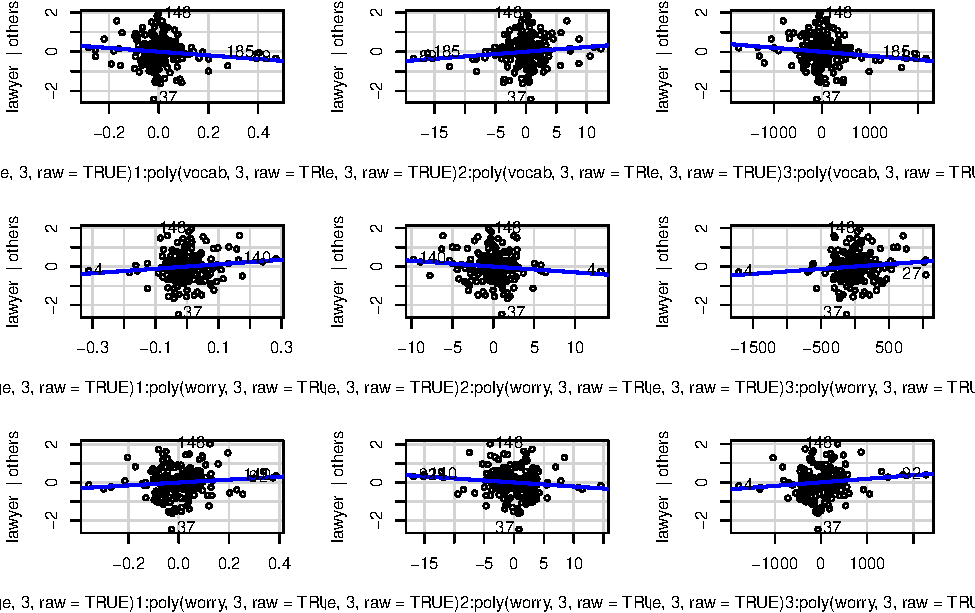
\includegraphics{HW5-Trinath-Sai-Subhash-Reddy-Pittala_files/figure-latex/unnamed-chunk-22-4.pdf}
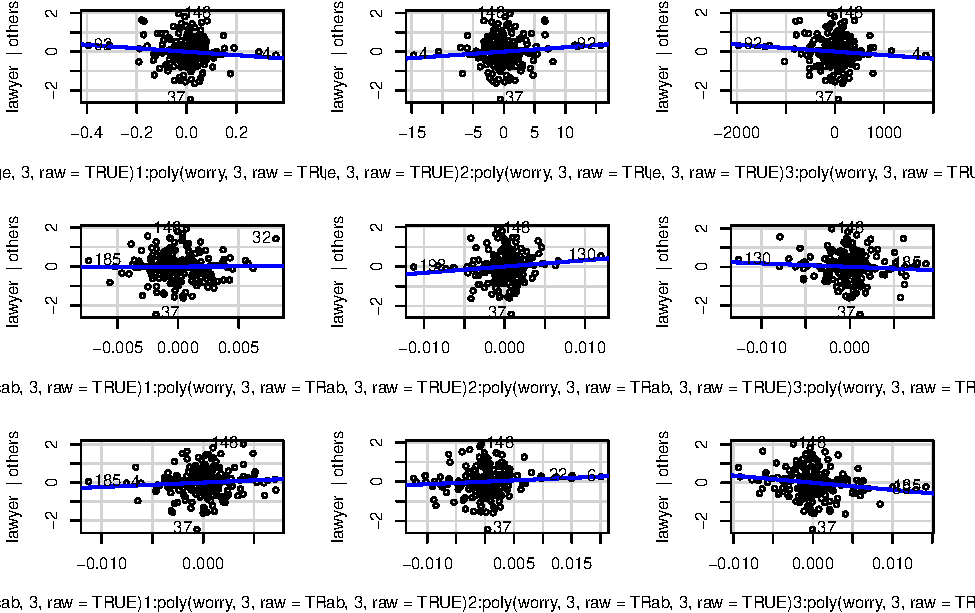
\includegraphics{HW5-Trinath-Sai-Subhash-Reddy-Pittala_files/figure-latex/unnamed-chunk-22-5.pdf}
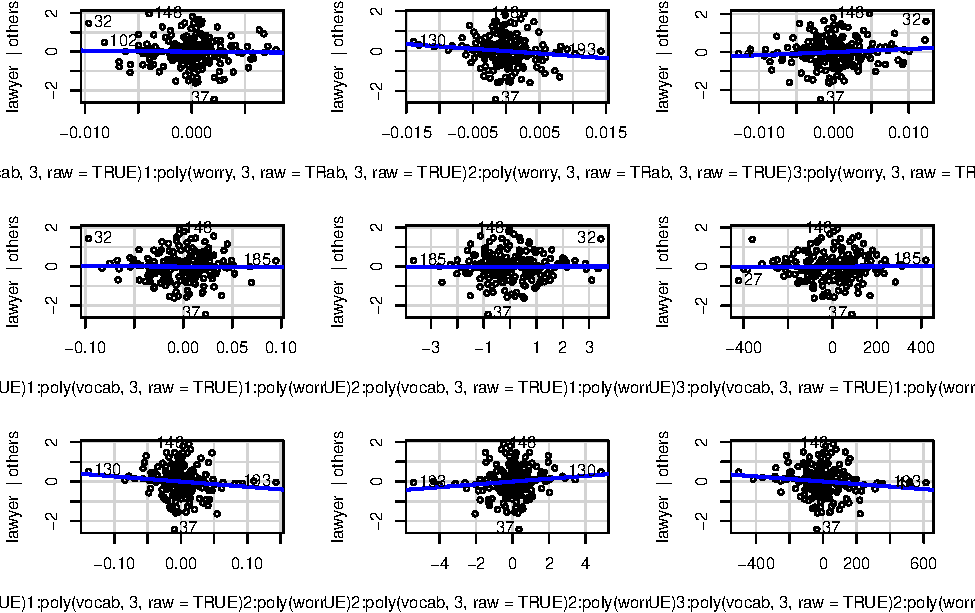
\includegraphics{HW5-Trinath-Sai-Subhash-Reddy-Pittala_files/figure-latex/unnamed-chunk-22-6.pdf}
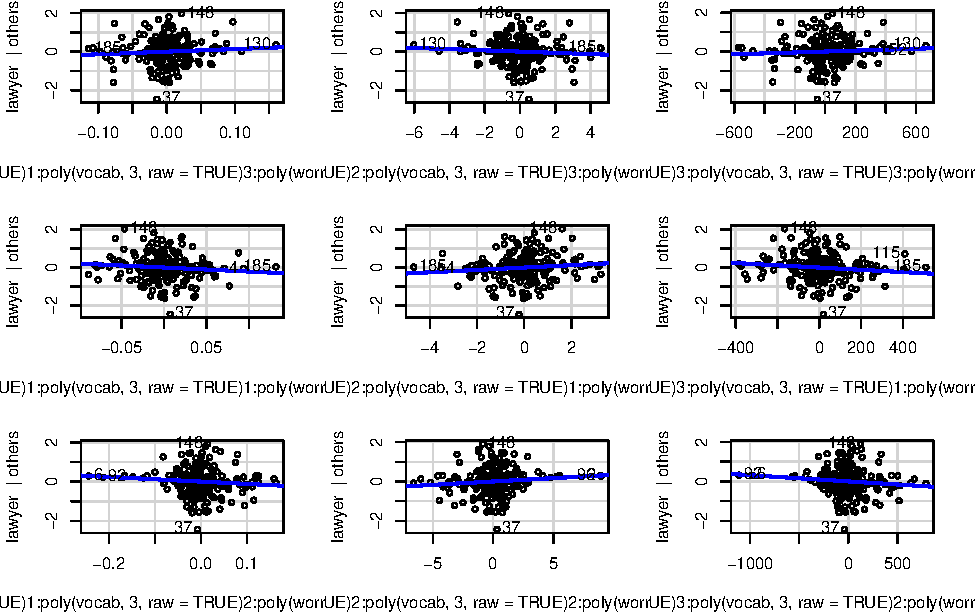
\includegraphics{HW5-Trinath-Sai-Subhash-Reddy-Pittala_files/figure-latex/unnamed-chunk-22-7.pdf}
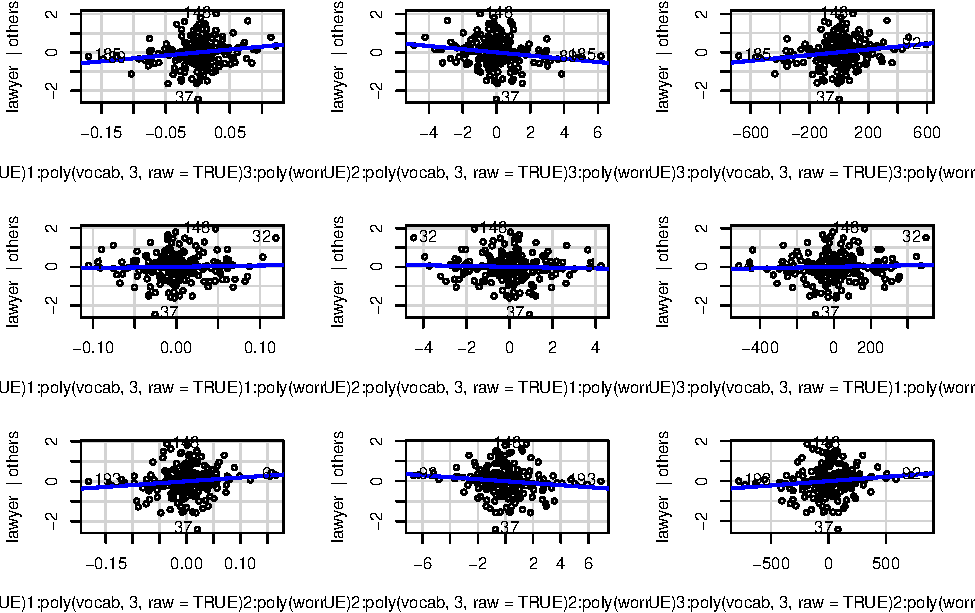
\includegraphics{HW5-Trinath-Sai-Subhash-Reddy-Pittala_files/figure-latex/unnamed-chunk-22-8.pdf}
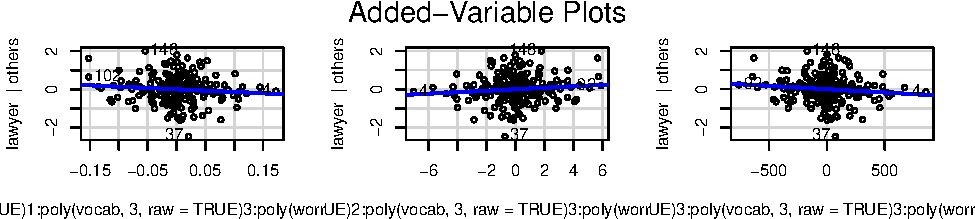
\includegraphics{HW5-Trinath-Sai-Subhash-Reddy-Pittala_files/figure-latex/unnamed-chunk-22-9.pdf}

\begin{Shaded}
\begin{Highlighting}[]
\FunctionTok{autoplot}\NormalTok{(M2\_archtct\_step)}
\end{Highlighting}
\end{Shaded}

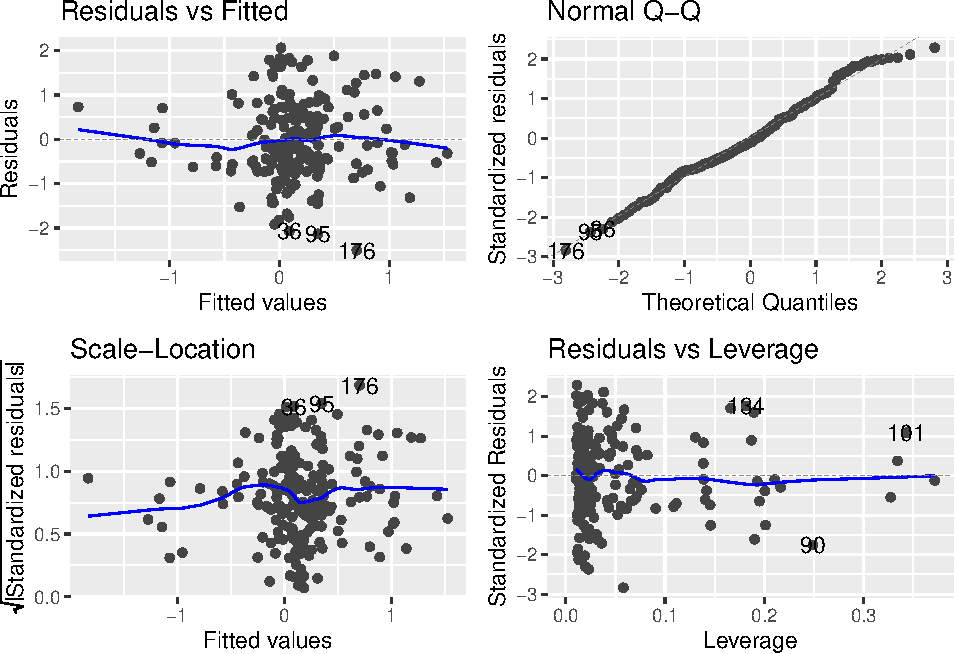
\includegraphics{HW5-Trinath-Sai-Subhash-Reddy-Pittala_files/figure-latex/unnamed-chunk-23-1.pdf}

\begin{Shaded}
\begin{Highlighting}[]
\FunctionTok{avPlots}\NormalTok{(M2\_archtct\_step)}
\end{Highlighting}
\end{Shaded}

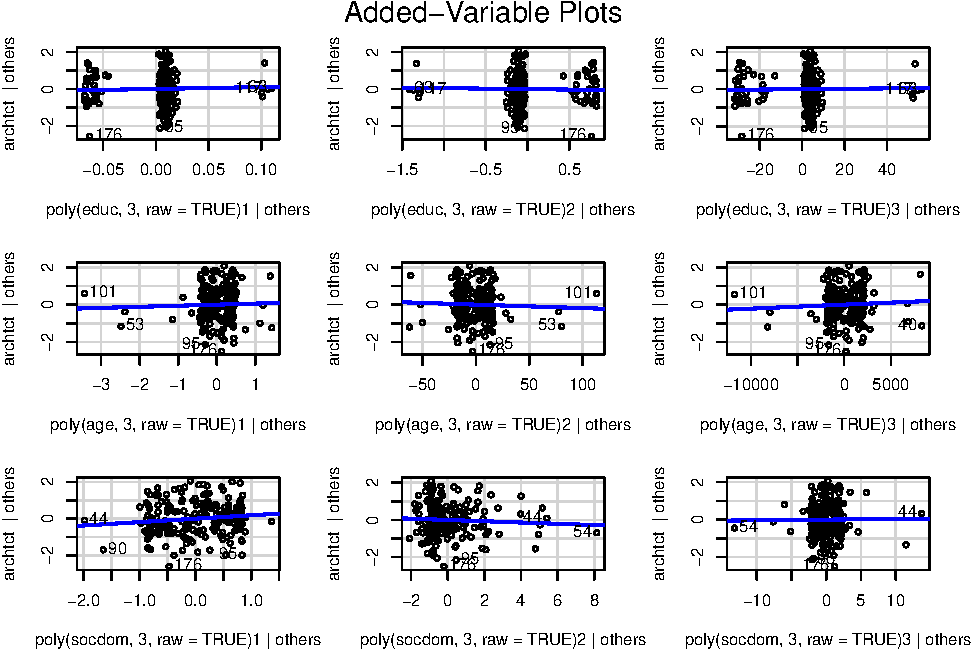
\includegraphics{HW5-Trinath-Sai-Subhash-Reddy-Pittala_files/figure-latex/unnamed-chunk-23-2.pdf}

\end{document}
